\begin{center}
\Huge
Aflevering om eksponentialfunktioner og eksponentiel vækst
\end{center}
\section*{Opgave 1}
\stepcounter{section}
To funktioner $f$ og $g$ er givet ved henholdsvist
\begin{align*}
f(x) = 0,7 \cdot (1,04)^x \textnormal{ og } g(x) = 1,2 \cdot (0,47)^x.
\end{align*}
\begin{enumerate}[label=\roman*)]
\item Hvilke typer funktioner er $f$ og $g$? 
\item Hvad er fremskrivningsfaktoren og vækstraten for de to funktioner?
\item Hvor skærer de to funktioner $y$-aksen?
\item Er funktionerne voksende eller aftagende?
\item Hvilken type funktion er produktet af de to funktioner $f\cdot g$? Bestem skæringen med $y$-aksen for $f\cdot g$.
\end{enumerate}

\section*{Opgave 2}
\stepcounter{section}
Graferne for tre eksponentialfunktioner $f$, $g$ og $h$ er tegnet på Fig. \ref{fig:tregraf}. Forskrifterne for funktionerne er
\begin{align*}
f(x) &= 2^x,\\
g(x) &= 2\cdot 2^x,\\
h(x) &= 2\cdot(0.5)^x.
\end{align*}
\begin{figure}[H]
\centering
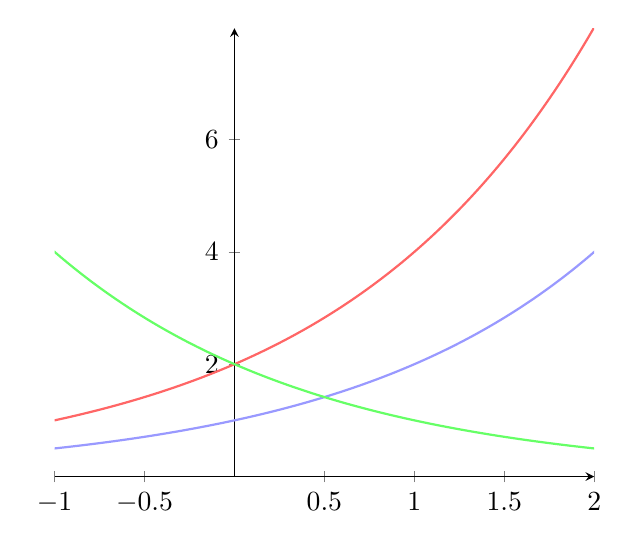
\begin{tikzpicture}
\begin{axis}[axis lines= middle, 
xmin  = -1,
xmax = 2,
ymin = 0,
]
\addplot[thick,samples = 1000,color=blue!40]{2^x};
\addplot[thick,samples = 1000,color=red!60] {2*2^x};
\addplot[thick,samples = 1000,color=green!60] {2*(0.5)^x};
\end{axis}
\end{tikzpicture}
\caption{Grafer for de tre funktioner $f$, $g$ og $h$.}
\label{fig:tregraf}
\end{figure}
\begin{enumerate}[label=\roman*)]
\item Par funktionerne $f$, $g$ og $h$ med graferne på Fig. \ref{fig:tregraf}. Argumentér ved at bruge betydningen af konstanterne $a$ og $b$ for funktionerne.
\end{enumerate}

\section*{Opgave 3}
\stepcounter{section}
I Tabel \ref{tab:tab1} er to datapunkter givet.
\begin{table}[H]
\centering
\begin{tabular}{c|c|c}
$x$ & 2 & 5\\ \hline
$y$ & 18 & 486
\end{tabular}
\caption{To punkter}
\label{tab:tab1}
\end{table}
\begin{enumerate}[label=\roman*)]
\item Brug topunktsformlen for eksponentialvækst til at bestemme forskriften til den eksponentialfunktion $f$ , der skærer de to punkter. 
\item Bestem fordoblingskonstanten/halveringskonstanten for $f$.
\item Tag den naturlige logaritme $\ln$ af $y$-værdierne. Dette kan ses af Tabel \ref{tab:tab2}.
\begin{table}[H]
\centering
\begin{tabular}{c|c|c}
$x$ & 2 & 5\\ \hline
$y$ & $\ln(18)$ & $\ln(486)$
\end{tabular}
\caption{$\ln$-transformation af punkter}
\label{tab:tab2}
\end{table}
\item Brug topunktsformlen for lineære funktioner på disse punkter. Du får så et udtryk $y = a\cdot x + b$. 
\item Bestem $e^{a}$ og $e^b$. Sammenlign med fremskrivningsfaktoren og skæringen med $y$-aksen for $f$. 
\end{enumerate}


\section*{Opgave 4}
\stepcounter{section}
Tabel \ref{tab:tab3} beskriver antallet af bakterier $N$ i en opløsning efter tid $t$. Enheden for $N$ er mio. bakterier og $t$ er tid i timer. 
\begin{table}[H]
\centering
\begin{tabular}{c|c|c|c|c|c|c|c|c|c|c|c|c}
$t$ & 0 & 1 & 2 & 3 & 4 & 5 & 6 & 7&8&9&10&11\\ \hline
$N(t)$ & 2,8 & 3 & 3 & 3,4 & 3,7 & 4,2 & 4,7 & 4,8 & 5,8 & 6,4 & 7,5 & 9,2
\end{tabular}
\caption{Bakterievækst}
\label{tab:tab3}
\end{table}
\begin{enumerate}[label=\roman*)]
\item Bestem den eksponentialfunktion $\hat{N}$, der passer bedst på datasættet Tabel \ref{tab:tab3}.
\item Hvad er fremskrivningsfaktoren for $\hat{N}$? Hvad med skæringen med $y$-aksen?
\item Bestem fordoblingskonstanten for $\hat{N}$, og fortæl, hvad den betyder for modellen af bakterievæksten.
\item Hvor mange bakterier fortæller modellen os, at der er efter et døgn? Hvad med en uge? 
\item Kan vi forvente, at denne model bliver ved med at beskrive den rigtige bakterievækst $N(t)$ for evigt?